\documentclass[10pt,a4paper]{article}
\usepackage[utf8]{inputenc}
\usepackage{amsmath}
\usepackage{amsfonts}
\usepackage{amssymb}
\usepackage{listings}
\usepackage{graphicx}
\lstset{showstringspaces=false}
\begin{document}
\title{Intelligent Systems Assignment 1}
\author{Wessel Becker (1982362) \& Sander ten Hoor (2318555)}
\maketitle
\section{MatLab code}
\subsection{Changes to tsp.m}
The decrease T by 0.1\% was removed.

\lstinputlisting[language=Matlab, firstline=27, lastline=29]{./Salesman/tsp.m}
\subsection{plotmean.m}
\lstinputlisting[language=Matlab]{./Salesman/plotmean.m}

\section{Plots}
To show the impact of T, several T values have been used to run the tsp function. The tsp function returns the generated distance values. The last fifty of these values are used to plot the mean against the used T value.

These plots show the value of T on the x-axis against the mean on the y-axis. The standard deviation is displayed around the data points.

\makebox[\textwidth]{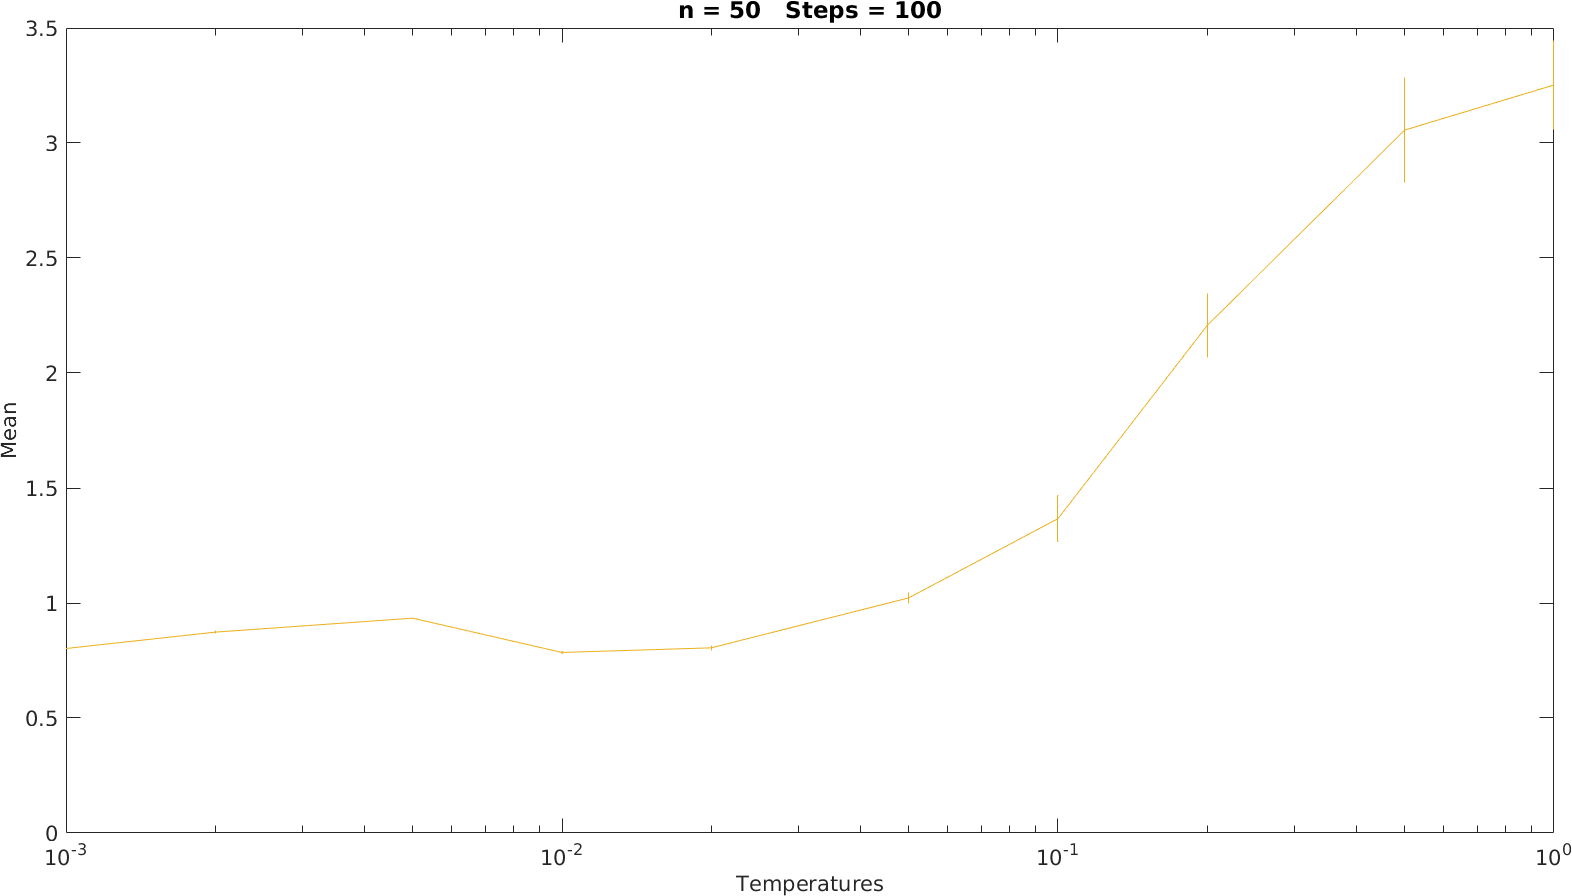
\includegraphics[width=\paperwidth]{./Salesman/n50s100}} \\
In this graph, the standard deviation is quite high with higher temperatures, and declines together with the mean. 

\makebox[\textwidth]{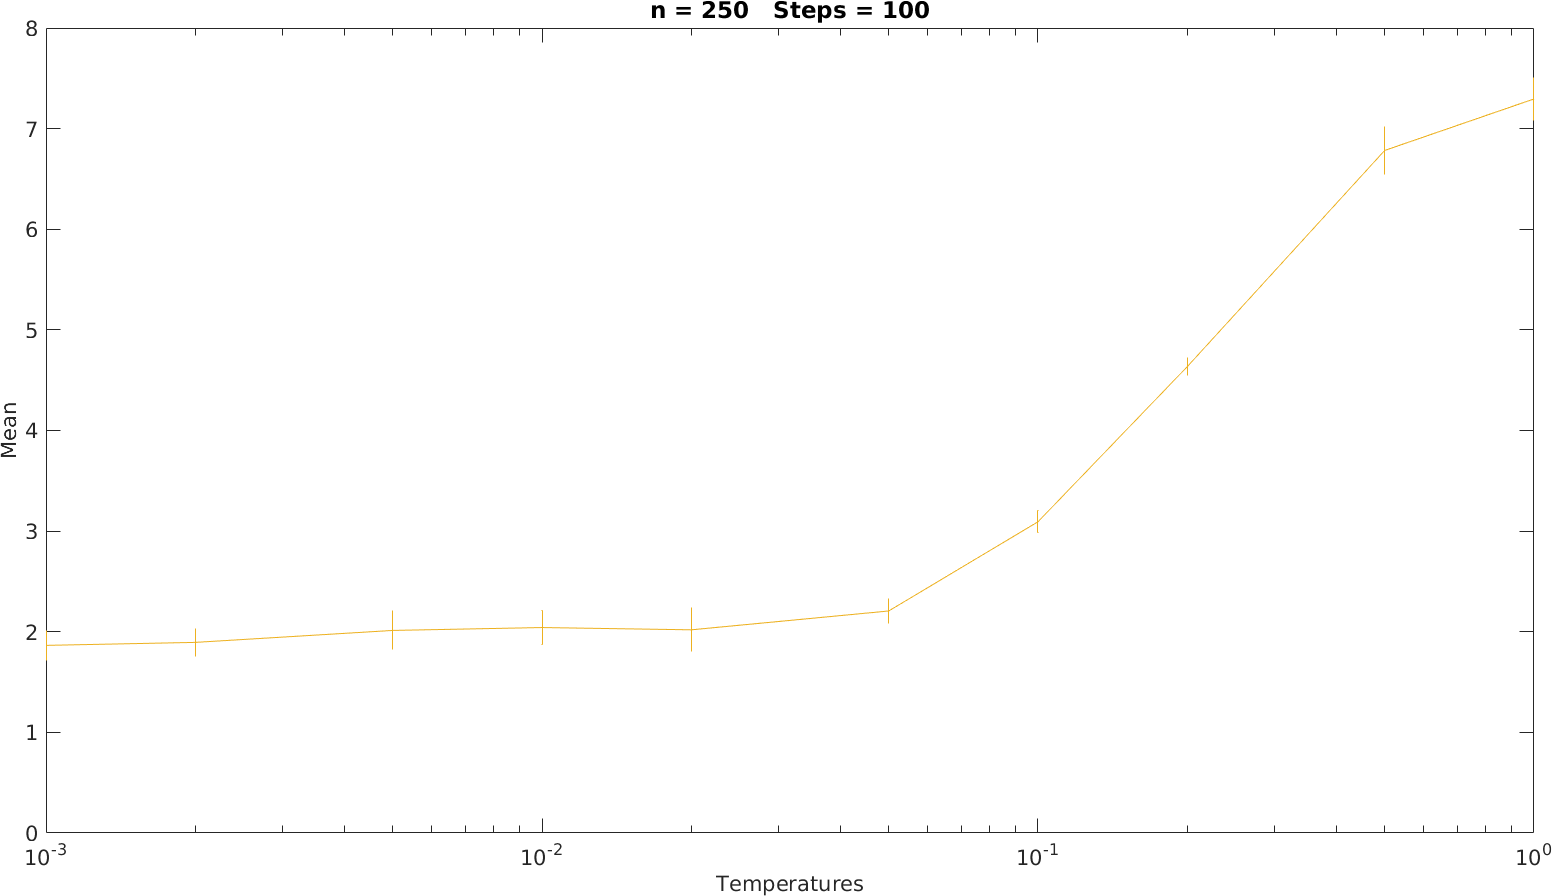
\includegraphics[width=\paperwidth]{./Salesman/n250s100}} \\
Increasing the amount of cities from 50 to 250 also shows an increase of the mean (the y-axis has increased to 8 from 4 to accomodate for the mean) and the standard deviation.

\makebox[\textwidth]{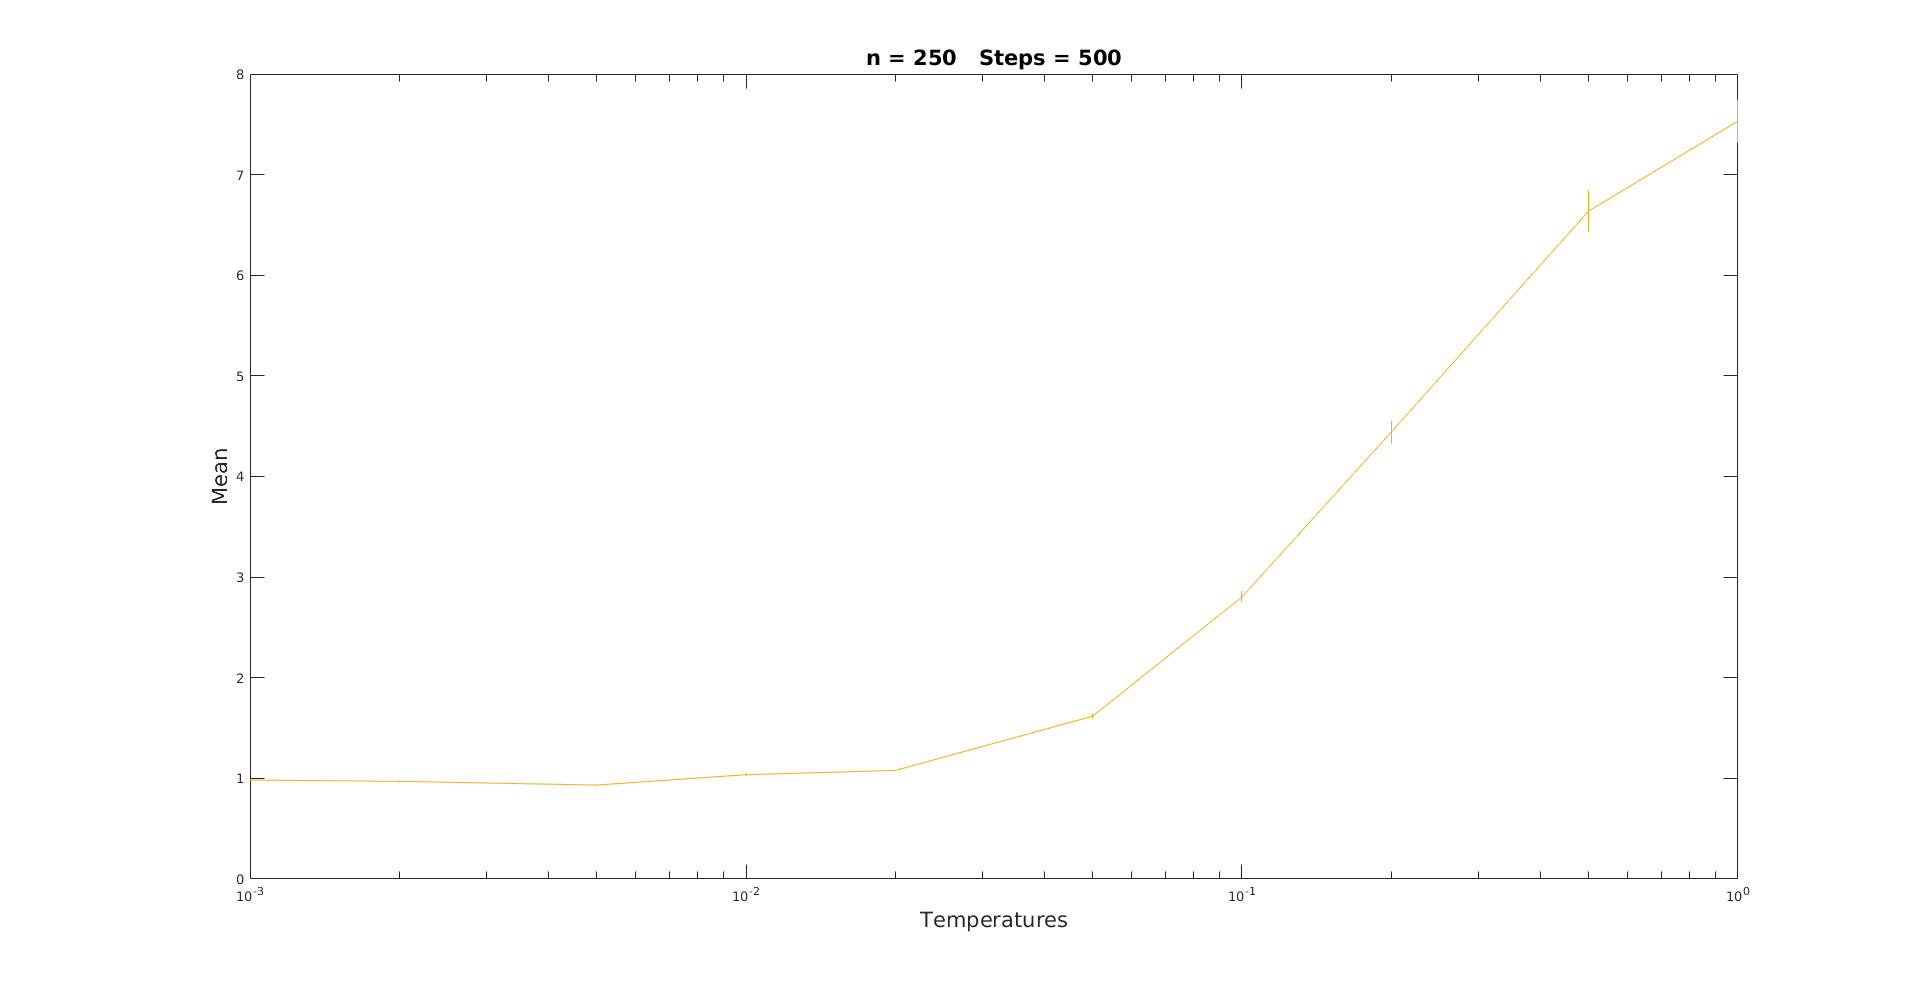
\includegraphics[width=\paperwidth]{./Salesman/n250s500}} \\
By keeping the number of cities (250) but increasing the number of steps to 500, the mean and the standard deviation decrease again. The latter decreases so much it is difficult to see near the lower temperatures.

\makebox[\textwidth]{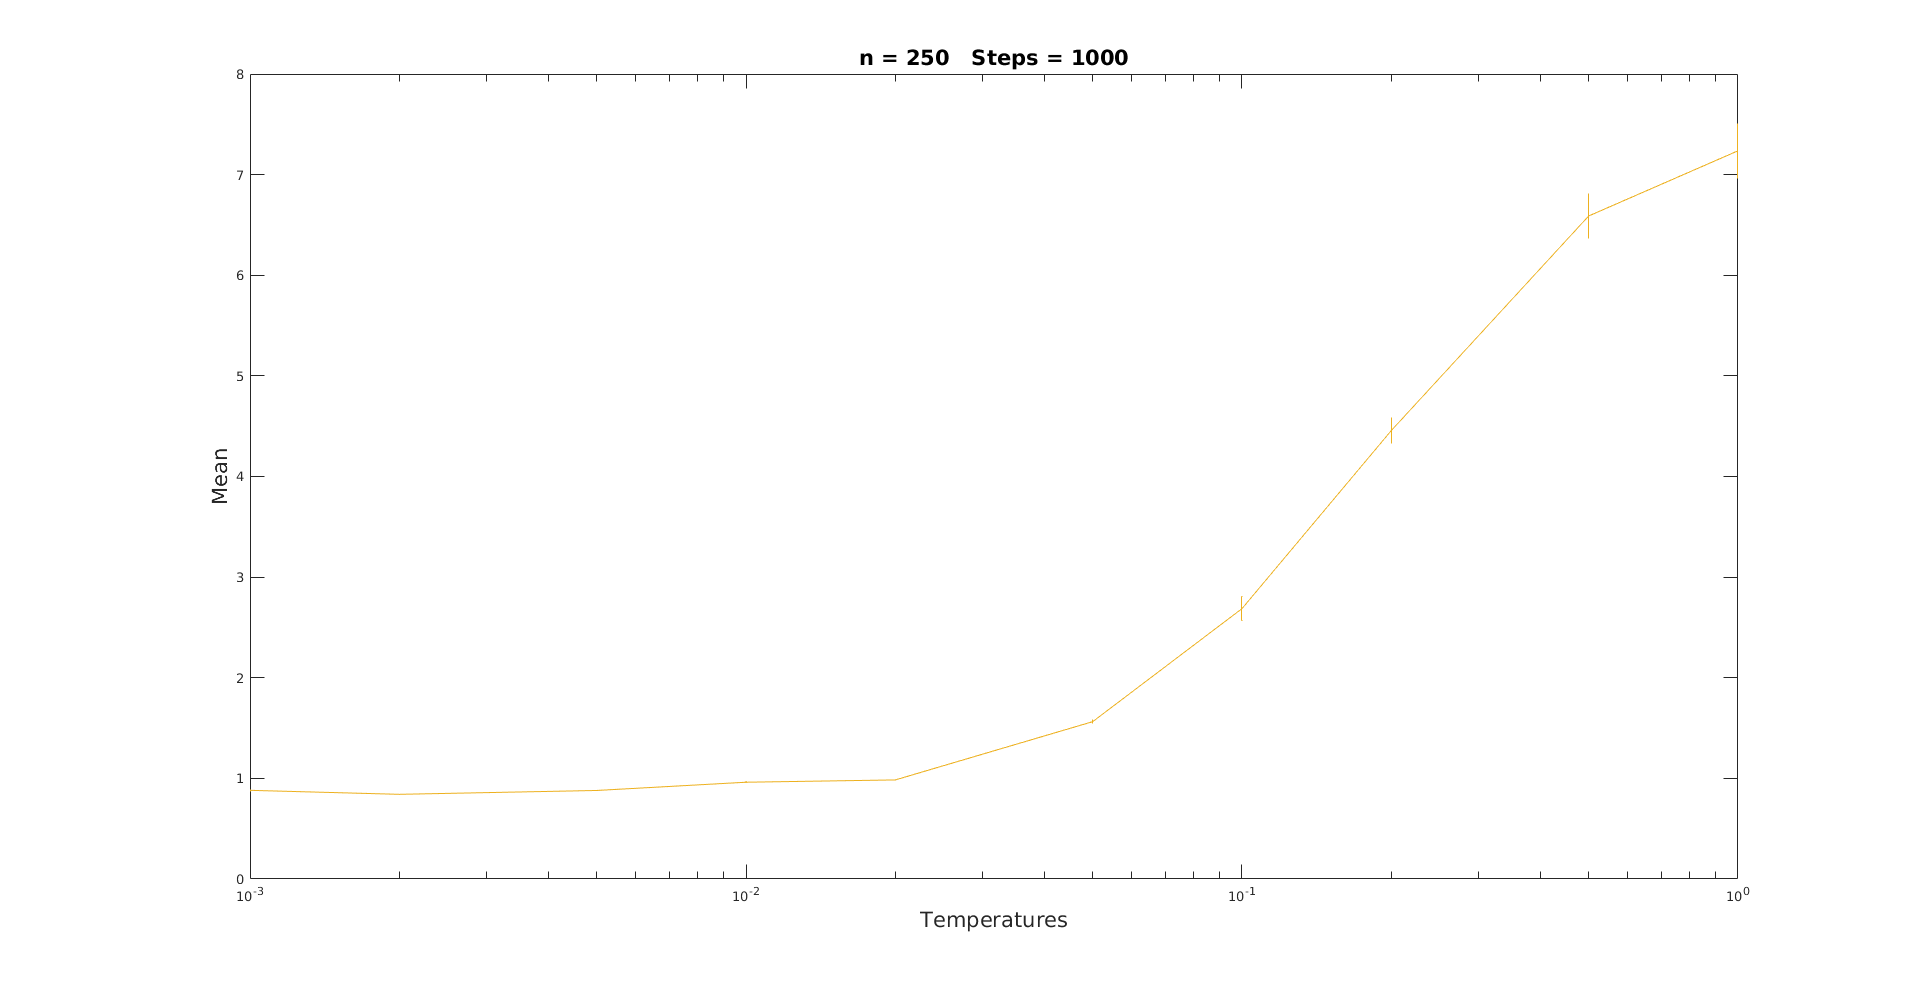
\includegraphics[width=\paperwidth]{./Salesman/n250s1000}} \\
Increasing the number of steps even further, doubling it to 1000, the mean only becomes slightly lower. The standard deviation becomes difficult to spot one temperature earlier.

\makebox[\textwidth]{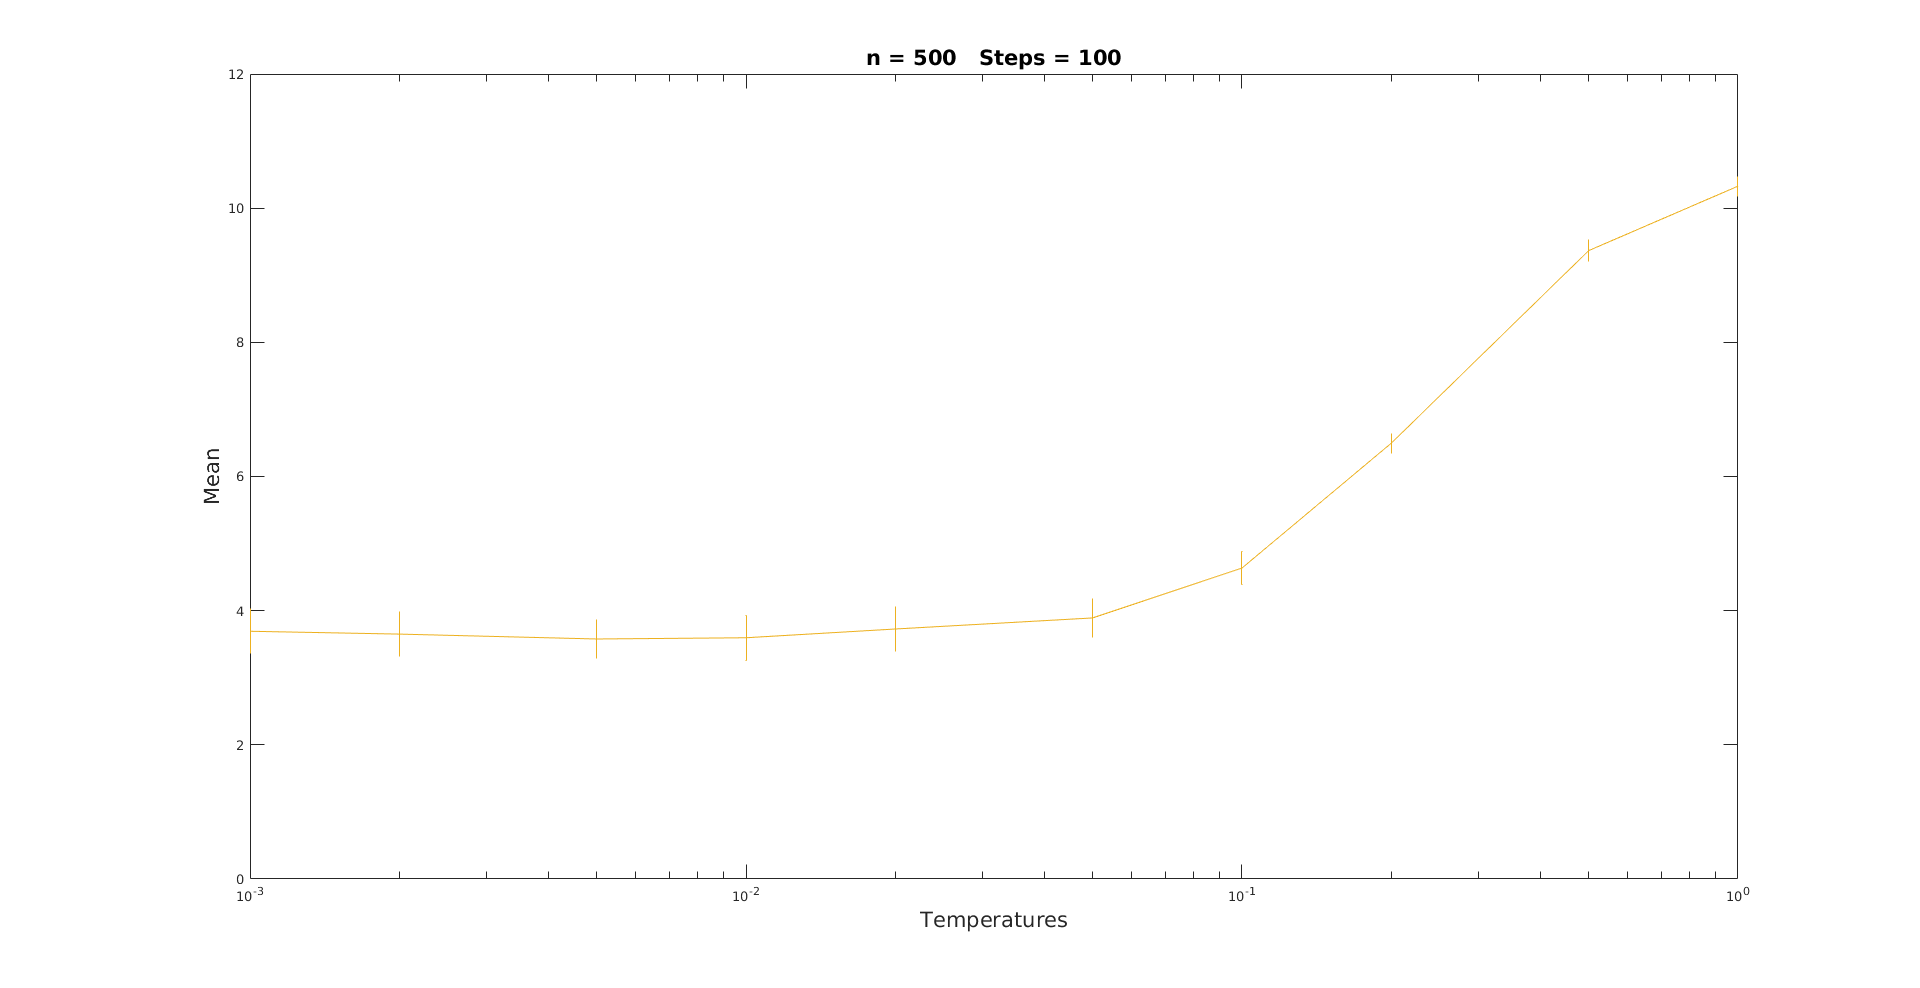
\includegraphics[width=\paperwidth]{./Salesman/n500s100}} \\
Increasing the number of cities to 500, but only taking 100 steps results in this plot. The mean is higher than in the other plots, and the standard deviation.

\section{T-Dependance}
-Correlation of T and the resulting mean distance?
-
\section{Work done}
The MatLab code was written by Sander and refactored by Wessel. 
\end{document}